\chapter{Robot Operating System - ROS}\label{cap:ros}

\begin{citacao}
``O Robot Operating System (ROS) é um conjunto de bibliotecas de software e ferramentas que te auxiliam na construção de aplicações em robótica. De \textit{drivers} ao estado da arte de algoritmos, e com poderosas ferramentas de desenvolvimento, ROS tem o que você precisa para seu próximo projeto de robótica. E tudo é open source~\cite{Ros}''    
\end{citacao}

O ROS foi idealizado com o objetivo de ser um ambiente completo, de código aberto, para elaboração de sistemas robóticos. Largamente aceito e amplamente utilizado atualmente, os desenvolvedores se beneficiam da alta qualidade de código proporcionado pelo grande número de usuários e plataformas que aproveitam-se do ROS em seus projetos~\cite{RosIntro}. Uma ampla variedade de sensores e atuadores empregados na robótica também seguem essa tendência e oferecem suporte ao ROS através de seus~\textit{drivers}. O ROS fornece abstração de hardware, controle de baixo nível para dispositivos, funcionalidades e bibliotecas de uso comum, passagem de mensagens entre processos e gerenciamento de pacotes~\cite{rosEfetiveProgram}. Por esses motivos, o ROS é conhecido como um meta sistema operacional para robôs. Neste capítulo será apresentado o ROS e as vantagens do seu uso na concepção de novas plataformas robóticas.

A cada ano o ROS vem se consolidando como o~\textit{framework} padrão para o desenvolvimento de novos projetos de robótica. Apesar de já possuir esta posição, o ROS possui uma história relativamente curta. O ROS teve início no Laboratório de Inteligência Artificial de Standord e em 2007 a companhia Willow Garage assumiu o seu desenvolvimento. A Willow Garage é uma empresa que desenvolve robôs pessoais e de serviços. Ela também é responsável pelo desenvolvimento de suporte a \textit{Point Cloud Library (PCL)}, que é uma biblioteca de software largamente usada para processamento de nuvens de pontos. Em Janeiro de 2010 a primeira versão do ROS foi lançada, desde então muitas outras versões a sucederam. O ROS está sob as licenças BSD 3-Clause e Apache 2.0, que permite qualquer um modificar, reusar e distribuir códigos ROS~\cite{rosPYO}. Atualmente o ROS se encontra com uma versão estável do ROS2 e o ROS1 tem seu fim marcada para maio de 2025.


\section{Um sistema operacional para robôs}

De forma simplificada um sistema operacional tem como objetivo gerenciar os recursos do sistema computacional, ele atua como uma ponte entre esses recursos e o seu usuário, ou seja, o sistema operacional se faz necessário para disponibilizar às aplicações os recursos funcionais do sistema de forma padronizada, se tornando uma verdadeira camada de abstração entre os programas e o hardware. Windows e Ubuntu, para computadores pessoais, e Android, para smartphones, são exemplos de sistemas operacionais populares.

A comunidade da robótica em todo mundo tem feito grande progresso nos últimos anos. Dispositivos de hardware confiáveis e com menor custo têm sido ofertados em um nível nunca encontrado no passado, desde robôs móveis terrestres, passando por drones e até mesmo robôs humanóides estão disponíveis no mercado com relativa facilidade. O que pode ser até mais impressionante, a comunidade também tem desenvolvido algoritmos que permitem que estes robôs possuam um nível crescente de autonomia. Apesar desse rápido progresso, o desenvolvimento de robôs ainda representam um desafio para os desenvolvedores de software e grande parte desse desafio se deve a falta de padronização de um software específico para robótica, ou até mesmo um sistema operacional dedicado para robôs, como podemos encontrar em outros nichos, como os PCs e smartphones. Neste contexto, o ROS tenta preencher essa lacuna.

O nome ROS vem da abreviação de \textit{Robot Operating System}, mas seria o ROS um sistema operacional para robôs? Ele fornece abstração de hardware, controle de baixo nível para dispositivos, implementações de funcionalidades de uso comum, troca de mensagens entre processos, até um sistema de gerenciamento de pacotes. Além destas características o ROS está equipado com bibliotecas e ferramentas para escrever, compilar e rodar seus códigos~\cite{RosIntro}.

Apesar de todos os atributos que o caracterizam como um sistema operacional, o ROS não é um sistema operacional convencional, por ainda precisar rodar em um outro sistema operacional previamente instalado, o que faz com que o ROS seja conhecido como um meta-sistema operacional. Antes de ter o ROS em execução no robô é necessário instalar um sistema operacional, como por exemplo o Ubuntu. Com a distribuição Linux rodando é possível executar a instalação completa do ROS, sendo assim, todos os recursos fornecidos por um sistema operacional convencional podem ser utilizados pelo ROS, como sistema de gerenciamento de processos, sistema de arquivos, interface do usuário e compiladores, dentre outros. 

Para complementar esses recursos básicos do sistema operacional, o ROS fornece funcionalidades específicas para o uso na robótica, tal como bibliotecas para transmissão e recepção de dados para uma variedade de dispositivos de hardwares comumente utilizados em sistemas robóticos. Esse tipo de software é conhecido como \textit{middleware} ou \textit{framework}. Como pode ser visto na Figura~\ref{fig:rosmeta}, o ROS é o sistema auxiliar para controlar atuadores e sensores, com um nível de abstração de hardware dando suporte para o desenvolvimento de novas aplicações de robótica em sistemas operacionais convencionais.

\begin{figure}[ht]
	\caption{ROS: um meta-sistema operacional}
	\begin{center}
		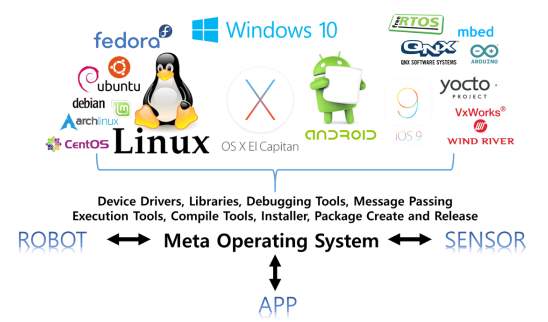
\includegraphics[scale=0.6]{imagens/metaOS.png}\\
		{\small \textbf{Fonte:} \citeonline{rosPYO}}
    \end{center}\label{fig:rosmeta}
\end{figure}


\section{Vantagens do ROS}
Até agora descrevemos o ROS como uma ferramenta ideal para o desenvolvimento de novos projetos de robótica, apesar disto, aprender a usar um novo \textit{framework} é uma atividade árdua, principalmente um tão abrangente e complexo como o ROS\@. Esse tipo de questão deve ser levada em consideração na escolha das ferramentas no inicio de um novo projeto. 

O objetivo do ROS não é ser um \textit{framework} com o maior número de recursos, seu principal objetivo é oferecer o máximo de reuso de software usados no desenvolvimento de novos robôs. O ROS é um \textit{framework} de computação distribuída, isso que dizer que os seus processos podem ser projetados individualmente e podem ser integrados ao sistema livremente e em tempo de execução. Estes processos podem ser agrupados em pacotes, facilitando o compartilhamento e a sua distribuição. Outra iniciativa para incentivar a colaboração e o compartilhamento de código são os repositórios oficiais do ROS, que estão disponíveis de forma livre. 

A seguir serão listadas algumas características que incentivam a colaboração da comunidade e são responsáveis pelo sucesso do ROS\@:

\begin{itemize}
    \item\textbf{Recursos Nativos:} O ROS oferece, de forma nativa, muitos recursos prontos, testados e validados pela comunidade. Podemos citar como exemplos o \textit{Simultaneous Localization and Mapping (SLAM)} e o \textit{Adaptive Monte Carlo Localization (AMCL)} que são usados para navegação autônoma de plataformas robóticas móveis. Outro pacote oferecido pelo ROS é o MoveIt, pacote usado para planejamento de movimento de manipuladores. Estes recursos podem ser usados sem problema algum e são altamente configuráveis, podendo ser adaptados em vários modelos de robôs e atender a inúmeras aplicações. 

    \item\textbf{Ferramentas de desenvolvimento:} O ROS é disponibilizado com uma grande quantidade de ferramentas para debugging, visualização, incluindo ferramentas para simulação. Algumas das ferramentas open source mais poderosas para visualização, debugging e  simulação, respectivamente, rqt\underline{ }gui, RViz e Gazebo, são nativas do ambiente ROS\@.
    
    \item\textbf{Suporte a sensores e atuadores:} Muitos dos sensores e atuadores usados na robótica já são suportados pelo ROS e o número de dispositivos compatíveis aumenta a cada ano. Algumas companhias se beneficiam pelo fato de muitos desses dispositivos fazerem uso de hardware aberto e o software existente também pode ser reutilizado a custo zero, fazendo com que o processo de desenvolvimento de novos hardware periféricos usados na robótica também acelere. Sensores como Velodyne-LIDAR e atuadores como os servos Dynamixel, podem ser integrados ao ROS sem impedimento algum.
    
    \item\textbf{Múltiplas linguagens:} O framework ROS pode ser programado em algumas linguagens de programação modernas. Podemos escrever código eficiente em C ou C++ e outra aplicação ser escrita em python. O ROS possui bibliotecas clientes para C/C++, Python, Java e Lisp. Este tipo de flexibilidade não é comum em outros \textit{frameworks}.
    
\end{itemize}


\subsection{Computacão distribuida}
Grande parte de robôs modernos possuem diferentes unidades de processamento, que podem estar localizadas em diferentes computadores. Desde sensores microprocessados até mesmo controles específicos para motores, tais dispositivos podem possuir suas próprias unidades computacionais. Mesmo possuindo apenas um computador, dividir o processamento em processos individuais específicos para cada função e fazer com que eles trabalhem em conjunto na resolução de um problema maior, é uma excelente abordagem para a arquitetura de robôs modernos. Além disso, múltiplos robôs podem trabalhar de forma colaborativa dividindo atividades entre eles, ou até mesmo interagindo com seres humanos que poderiam enviar comandos através de um computador ou celular. Em todos estes casos, é necessário a comunicação entre processos, que podem ou não estarem no mesmo computador. 

O ROS é um \textit{Inter-process communication framework} e de fato ele usa uma rede TCP/IP para realizar essa comunicação entre processos. Ele usa sockets TCP/IP para transportar dados entre os processos. Esta abordagem proporciona grande flexibilidade na troca de mensagem: processos podem se comunicar com outros mesmo se eles não estiverem na mesma máquina, ou até mesmo em robôs separados, bastando para tal que todas as máquinas que compartilham estejam na mesma rede. Isso faz com que até mesmo processos rodando na internet possam participar da comunicação e realizar uma parte do processamento de um robô.


\subsection{Reuso de Software}
O uso do ROS pode diminuir a necessidade de implementar algoritmos que já foram testados e validados por outros pesquisadores. Algoritmos de navegação, planejamento de rotas e mapeamento, dentre outros, são usados em diferentes projetos, e o ROS permite que estes algoritmos sejam reaproveitados de duas maneiras possíveis:

\begin{itemize}
    \item \textbf{Pacotes padrão:} São pacotes de software de importantes algoritmos usados na robótica ou mesmo drivers de dispositivos comuns na robótica, que já foram implementados e testados.

    \item \textbf{Interface de troca de mensagens:} A interface utilizada pelo ROS vem se tornando um padrão na comunicação entre processos em robôs.
\end{itemize}

Nos repositórios oficiais do ROS, estão disponíveis centenas de pacotes públicos que utilizam a interface de troca de mensagens padronizada do ROS, o que possibilitando uma redução significativa do esforço necessário para o desenvolvimento de uma integração destes pacotes ao seu sistema. Assin, desenvolvedores que usam o ROS podem concentrar mais tempo e esforços no desenvolvimento de suas novas ideias, aproveitando algoritmos consolidados dos repositórios oficiais do ROS, sem a necessidade de reescrevê-los para adaptá-los ao seu projeto.


\section{Sistema de aquivos}
Como era de se esperar de um sistema operacional, o ROS também possui um sistema de arquivos padronizado. É de extrema importância para o desenvolvimento de novas aplicações conhecer a organização dessa estrutura de arquivos. A Figura~\ref{fig:rosfile} apresenta um diagrama de blocos do sistema de arquivo do ROS\@.

\begin{figure}[ht]
	\caption{Sistema de arquivos ROS}
	\begin{center}
		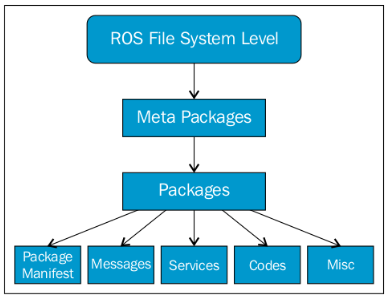
\includegraphics[scale=0.7]{imagens/fileSiystem.png}\\
		{\small \textbf{Fonte:} \citeonline{rosMastering}}
    \end{center}\label{fig:rosfile}
\end{figure}

A seguir são apresentadas as definições de cada bloco da estrutura de arquivos do ROS\@:
\begin{itemize}
    \item \textbf{Pacotes:} Pacotes são a unidade de software principal do ROS\@. Um pacote pode conter nós, dependências, bibliotecas, \textit{datasets}, arquivos de configuração, ou qualquer coisa que seja útil organizar de forma agrupada~\cite{RosPKG}.

    \item \textbf{Manifesto do pacote:} O arquivo package.xml é conhecido como manifesto do pacote, ele fornece os metadados a respeito do pacotes, incluindo nome, versão, descrição, licença, dependências e outras informações. Os padrões do package.xml são definidos no REP-0127.
    
    \item \textbf{\textit{Metapackages}:} Metapackages são pacotes especializados que serve apenas como representante de um grupo de outros pacotes relacionados entre si.
    
    \item \textbf{Manifesto do \textit{metapackage}:} O manifesto de um metapackage é semelhante ao manifesto de um pacote comum, a diferença entre eles é que no manifesto devemos incluir as dependências encontradas no mesmo repositório do meta package
    
    \item \textbf{Arquivo .msg:} É o arquivo de descrição de um tipo de mensagem, é armazenado no diretório meu\underline{ }pacote/msg/Mensagem.msg e define toda a estrutura de dados enviados a partir deste tipo de mensagem.
    
    \item \textbf{Arquivo .srv:} É o arquivo de descrição de um tipo de mensagem, é armazenado no diretório meu\underline{ }pacote/srv/Servico.msg e define toda a estrutura de dados enviados a partir deste tipo de serviço.
    
    \item \textbf{Repositórios:} Pacotes ROS são compartilhados usando algum tipo de sistema de controle de versão, como o gti. Cada repositório pode conter apenas um pacote ou um metapackage 
\end{itemize}


\subsection{Pacotes ROS}

A unidade básica para configuração do software no ROS é conhecida como pacote, isso quer dizer que todas as aplicações desenvolvidas para ROS são estruturadas como um pacote. Na Figura \ref{fig:rospacotestrut} podemos ter uma visão da estrutura típica de um pacote ROS

\begin{figure}[ht]
	\caption{Estrutura típica de um pacote ROS}
	\begin{center}
		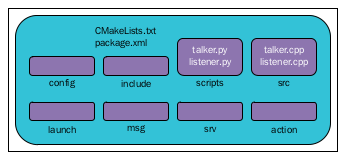
\includegraphics[scale=0.8]{imagens/rospackagestruture.png}\\
		{\small \textbf{Fonte:} \citeonline{rosMastering}}
    \end{center}\label{fig:rospacotestrut}
\end{figure}

Nos pacotes estão contidos um ou mais nós, como são chamadas as unidades de processamento no ROS, ou ainda arquivos de configuração para a execução de nós de outros pacotes. Existem milhares de pacotes ROS oficiais e uma quantidade ainda maior de pacotes desenvolvidos por seus usuários. 

Cada \textit{metapackage} possui um arquivo chamado package.xml, o qual é responsável por reunir informações importantes sobre o pacote. Nele podemos encontrar o nome do pacote, seu autor, dependências e licença de uso. O sistema de compilação do ROS é o Catkin, o qual usa o CMake e o arquivo CMakeLists.txt que deve estar dentro da pasta de cada pacote com as suas instruções de compilação. 

Os pacotes são as menores unidades que podem ser compiladas no ROS, são também  a maneira com que podemos organizar o software para ser lançado. No caso dos pacotes oficiais do ROS, por exemplo, existe um pacote Debian, que são os pacotes utilizados pelo Ubuntu, para cada pacote ROS. Apesar do conceito ser semelhante, e mesmo que ao instalar um pacote Debian, você possa incluí-lo à sua lista de pacotes ao ROS instalado no sistema, os pacotes Debian e ROS não são equivalentes. 

A principal função dos pacotes é ser uma maneira funcional, de fácil configuração e um caminho descomplicado para possibilitar o reuso de software. De maneira geral, os pacotes ROS devem conter funcionalidades suficientes para serem úteis, mas não muito para torná-los muito grande e confusos, dificultando seu uso por outro software 


\subsection{Mensagens ROS}
Os nós do ROS podem publicar apenas dados de tipos predeterminados. Estes tipos são definidos usando uma linguagem de descrição de mensagens, conhecida como mensagens ROS\@. Esta simples descrição permite que as ferramentas do ROS gerem automaticamente o código fonte para mensagens para todas as linguagens aceitas no ROS\@. As descrições das mensagens são armazenadas no arquivo .msg localizado no subdiretório msg/ dentro de um pacote ROS\@.

Existem dois segmentos em um arquivo .msg, são eles: campos e constantes. Campos são os dados que serão enviados dentro da mensagens. Constantes define os valores, ou tipo de dados, que poderão ser usados em cada campo. Os tipos de mensagens são referenciados a partir do nome do seu respectivo pacote-como ilustração, podemos usar o arquivo de descrição geometry\underline{ }msgs/msg/Twist.msg, que será referencido como geometry\underline{ }msgs/Twist. 

O ROS possui um grande número de mensagens predefinidas, o que não impede que o programador escreva seus próprios arquivos .msg com a descrição de uma mensagem específica para atender a sua aplicação. A Tabela~\ref{tab:rostype} lista os tipos de dados padrão do ROS que podem ser usados na criação de novas mensagens: 

\begin{table}[ht]
	\caption{Estrutura típica de um pacote ROS }
    \begin{center}
        \begin{tabular}{llll}
        \hline
        \textbf{Primitive type} & \textbf{Serialization} & \textbf{C++} & \textbf{Python} \\ \hline\hline
        bool(1)     & unsigned8-bitint              & uint8\_t(2)  & bool            \\ 
        int8        & signed8-bitint                & int8\_t      & int             \\ 
        uint8       & unsigned8-bitint              & uint8\_t     & int             \\ 
        int16       & signed16-bitint               & int16\_t     & int             \\ 
        uint16      & unsigned16-bitint             & uint16\_t    & int             \\ 
        int32       & signed32-bitint               & int32\_t     & int             \\ 
        uint32      & unsigned32-bitint             & uint32\_t    & int             \\ 
        int64       & signed64-bitint               & int64\_t     & long            \\ 
        uint64      & unsigned64-bitint             & uint64\_t    & long            \\ 
        float32     & 32-bitIEEEfloat               & float        & float           \\ 
        float64     & 64-bitIEEEfloat               & double       & float           \\ 
        string      & asciistring(4)                & std::string  & string          \\ 
        time        & Secs/nsecs signed 32bit ints  & ros::Time    & rospy.Time      \\ 
        duration    &S ecs/nsecs signed 32bit ints  & ros::Duration& rospy.Duration  \\ \hline
        \end{tabular}
        \\{\small \textbf{Fonte:} \citeonline{rosLearning}}
    \end{center}\label{tab:rostype}

\end{table}


\subsection{Workspace ROS}
De forma geral, o \textit{workspace} é uma pasta no computador que contém todos os pacotes que estão sendo usados no desenvolvimento de uma nova aplicação. Estes pacotes contêm os arquivos fontes e o \textit{workspace} fornece um local para que os pacotes sejam compilados. O \textit{workspace} é bastante útil quando é necessário compilar vários pacotes ao mesmo tempo: todos os pacotes poderão estar contidos no mesmo \textit{workspace}, centralizando todo processo de desenvolvimento. Não existe um diretório específico para que o \textit{workspace} seja criado, logo, ele pode ser criado no local de preferência do desenvolvedor e sua equipe. Um \textit{workspace} típico é mostrado na Figura~\ref{fig:rosworkspace}. 

\begin{figure}[ht]
	\caption{Estrutura típica de workspace ROS}
	\begin{center}
		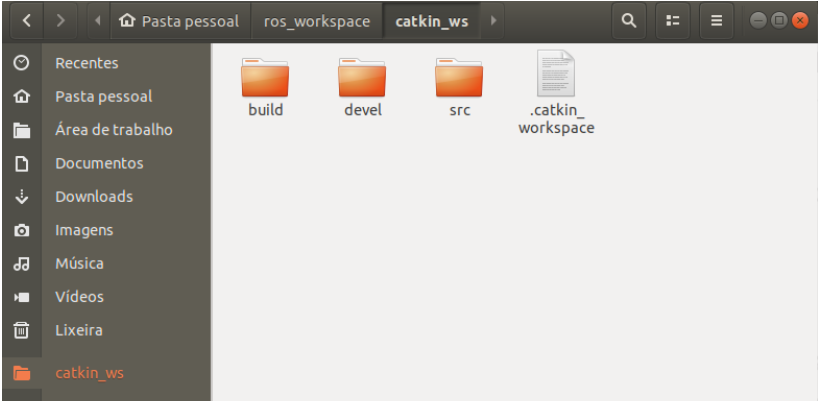
\includegraphics[scale=0.43]{imagens/rosworkspace.png}\\
		{\small \textbf{Fonte:} do Autor}
    \end{center}\label{fig:rosworkspace}
\end{figure}

Cada pasta dentro do workspace é um diferente espaço diferente, cada um com uma função específica:

\begin{itemize}
    \item \textbf{O espaço dos fontes:} No espaço dos fontes, localizada na pasta src do \textit{workspace}, estão localizados todos os pacotes do projetos. O arquivo mais importante dessa área do \textit{workspace} é o CMakeLists.txt. Este arquivo é gerado na primeira vez em que o \textit{workspace} é compilado

    \item \textbf{O espaço de compilação:} Localizado na pasta build, é neste local que são armazenadas as informações de cache, configurações e outros arquivos intermediários para que os pacotes sejam compilados corretamente.

    \item \textbf{O espaço de desenvolvimento:} Aqui são armazenados os programas compilados. Assim você pode testar seus programas sem a necessidade de instalá-los no sistema.
\end{itemize}

Outra função importante do ROS que pode ser usada através de um \textit{workspace} é o \textit{overlays}. Se você tiver um pacote instalado em seu sistema, mas quiser testar uma versão mais atual do mesmo pacote, não é necessário instalar a versão mais atual, você pode baixar o código fonte do pacote dentro do seu \textit{workspace}, após compilar o \textit{workspace} o ROS entende que deverá usar a versão presente no \textit{workspace} e não a versão instalada no sistema.


\section{Componentes ROS}

\subsection{Nós ROS}
No ROS os executáveis são chamados de nós, eles podem se comunicar com outros processos por meio dos tópicos, serviços ou pelo servidor de parâmetros. Os nós proporcionam grande modularidade aos sistemas robóticos que usam o ROS, isso faz com que o desenvolvimento destes sistemas se torne bem mais simples.

Ao ser executado, o nó possui um nome único no sistema, o que possibilita a sua comunicação com os demais nós. O ROS permite que os nós sejam escritos em diferentes linguagens de programação-as bibliotecas que fornecem a interface do ROS com uma linguagem específica são chamadas de clientes. As mais populares são: roscpp, para a linguagem C++ e a rospy para a linguagem Python.

Uma característica bastante interessante dos nós ROS é a possibilidade de parâmetros serem modificados no momento em que o nó é iniciado. Esta característica proporciona maior flexibilidade aos nós, já que o uso de parâmetros oferece a possibilidade de o código ser reconfigurado sem a necessidade de recompilar o código fonte, sendo assim podemos adaptar o nó a diferentes cenários sem conhecer detalhes de sua implementação. 


\subsection{Tópicos ROS}

Os tópicos são a maneira com que os nós enviam dados no ROS\@. Mesmo sem uma conexão direta entre dois nós, os tópicos podem ser transmitidos, fazendo com que a geração e o consumo de dados sejam desacoplados. Um tópico pode ser lido por vários nós e, de maneira igual, também pode ser publicado por vários nós, mas não é uma boa prática um mesmo tópico ser publicado por nós distintos, o que pode causar conflitos nas informações enviadas. A Figura~\ref{fig:rostopic} ilustra o processo de comunicação por meio de tópicos.

\begin{figure}[ht]
	\caption{Comunicação a partir de tópicos ROS}
	\begin{center}
		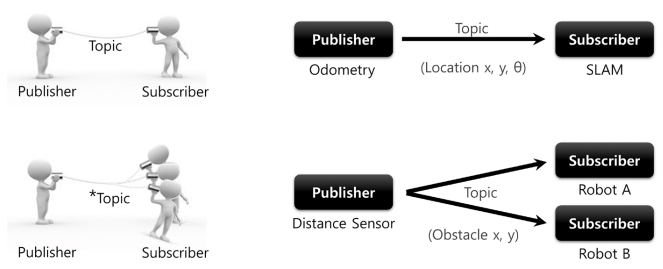
\includegraphics[scale=0.51]{imagens/rostopic.png}\\
		{\small \textbf{Fonte:} \citeonline{rosPYO}}
    \end{center}\label{fig:rostopic}
\end{figure}

As mensagens ROS são estruturas de dados simples que descrevem os tipos de dados que poderão ser transportados através dos tópicos. Isso faz com que os tópicos sejam fortemente tipados, consequentemente, o tipo de mensagem ROS deve ser o mesmo. Sendo assim, uma comunicação entre nós, por tópicos, ocorrerá se ambos, nó de leitura e nó de publicação, estiverem registrados no ROS \textit{master}, com tópicos de mesmo nome e mesmo tipo de mensagem ROS\@.


\subsection{ROS \textit{master}}

O ROS \textit{master} é o responsável por registrar nomes dos elementos que fazem parte do sistema, entre eles estão os nós, tópicos, serviços, action, tipos de mensagens, ele também é o encarregado por fornecer o servidor de parâmetros. Por gerenciar as informações das conexões entre as trocas de mensagens entre os nós, o \textit{master} é o primeiro elemento que deve ser executado no ROS. Afunção do \textit{master} é permitir que um determinado nó encontre outro, uma vez localizados os nós poderão se comunicar através de uma conexão per-to-per.

No momento em que um nós é executado no sistema, ele registra seu nome no \textit{master}. Sendo assim, o ROS \textit{master} possui os detalhes de todos os nós rodando no sistema. No momento em que qualquer detalhes de um nós muda, ele gera um callback para atualizar as novas informações no \textit{master}. Quando um nó inicia a publicação de um tópico ele informará todos os detalhes ao \textit{master}, desde do nome até o tipo de dados que serão enviado, em seguida, o \textit{master} verifica se existe algum outro nó lendo o mesmo tópico, se algum nó estão querendo fazer a leitura deste tópico o ROS \textit{master} irá compartilhar detalhes do nó que está publicando com o nós que quer ler o tópico.

Na Figura~/ref{fig:rosMastering} podemos ver como se da a interação entre o \textit{master} e os nós que farão a comunicação.


\begin{figure}[ht]
	\caption{Gerenciamento de comunicação através do ROS master}
	\begin{center}
		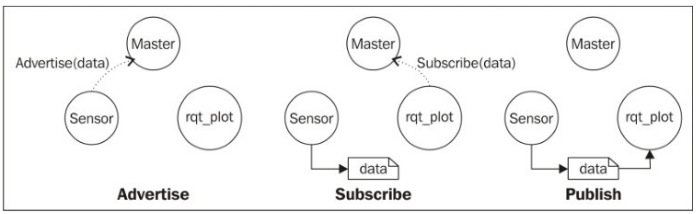
\includegraphics[scale=0.51]{imagens/rosmaster.png}\\
		{\small \textbf{Fonte:} \citeonline{rosEfetiveProgram}}
    \end{center}\label{fig:rosMastering}
\end{figure}

\subsection{ROS Parameters}

Parâmetros são variáveis globais que podem ser usadas por nós. Os parâmetros são criados com valores padrões, que podem ser lidos ou escritos por algum processo dentro do sistema ROS\@. O principal objetivo dos parâmetros é fornecer ao sistema a capacidade de se adaptar a cenários distintos de maneira ágil. Por exemplo, o desenvolvedor pode criar um nó para leitura de uma câmera USB, dando à esse nós parâmetros para que usuários desse nós possam configurar o frame rate em que os dados serão publicados, o nome da porta USB em que a câmera está conectada, entre outros, sempre ficando a critério do desenvolvedor. Em casos especiais os parâmetros poderão ser atualizados em tempo de execução, uma função muito útil principalmente em sistemas dinâmicos, que opera em constante mudança.
